\documentclass{beamer}
\usetheme{CambridgeUS}
\setbeamercolor{block title}{bg=red!80!black, fg=white}
\setbeamercolor{block body}{bg=red!10, fg=black}
%%%%%%%%%%%%%%%%%%%%%%%%%%%%%%%%%%%%%%%%%%%%%%%%%%%%%%%
\usepackage[utf8]{vietnam}
\usepackage{graphicx}
\usepackage{hyperref}
\usepackage{lipsum}
\usepackage{tikz}
%%%%%%%%%%%%%%%%%%%%%%%%%%%%%%%%%%%%%%%%%%%%%%%%%%%%%%%
% \AtBeginSection[]
% {
% \begin{frame}<beamer>
% \frametitle{Nội dung}

% \tableofcontents[
% currentsection,
% subsectionstyle=hide/hide,
% subsubsectionstyle=hide/hide
%]

% \end{frame}
%}
%%%%%%%%%%%%%%%%%%%%%%%%%%%%%%%%%%%%%%%%%%%%%%%%%%%%%%%
% \title[{\makebox[.15\paperwidth]{MI4100 - Mật mã và độ phức tạp thuật toán}}]{Chủ đề: Mô phỏng tấn công hệ mật mã khóa công khai RSA bằng thuật toán LLL giảm lưới}
% \author[Nhóm 8]{Nhóm 8}
% \date[\today]{\today}
%%%%%%%%%%%%%%%%%%%%%%%%%%%%%%%%%%%%%%%%%%%%%%%%%%%%%%%
\begin{document}
%%%%%%%%%%%%%%%%%%%%%%%%%%%%%%%%%%%%%%%%%%%%%%%%%%%%%%%
% % Trang tiêu đề
% % Cần có hình ảnh pictures/HUST2.jpeg
% % Không chỉnh sửa gì
% \begin{frame}
% \begin{tikzpicture}[remember picture, overlay]
% \node[anchor=center, inner sep=0pt] at (current page.center) {
\includegraphics[width=\paperwidth, height=\paperheight]{pictures/HUST2.jpeg}};
% \fill[white, opacity=0.8] (current page.south west) rectangle (current page.north east);
% \end{tikzpicture}
% \titlepage
% \end{frame}
%%%%%%%%%%%%%%%%%%%%%%%%%%%%%%%%%%%%%%%%%%%%%%%%%%%%%%%
% \begin{frame}{Danh sách thành viên}
% \begin{block}{Nhóm 8}
% \centering
% \begin{tabular} {|l|c|}
% \hline
% Họ và tên & MSSV \\
% \hline
% Vũ Văn Nghĩa & 20206205 \\
% Vũ Văn Nghĩa & 20206205 \\
% Vũ Văn Nghĩa & 20206205 \\
% Vũ Văn Nghĩa & 20206205 \\
% Vũ Văn Nghĩa & 20206205 \\
% \hline
% \end{tabular}
% \end{block}
% \end{frame}
%%%%%%%%%%%%%%%%%%%%%%%%%%%%%%%%%%%%%%%%%%%%%%%%%%%%%%%
% \begin{frame}{Phân công thành viên}
% \begin{block}{Phân công}
% \begin{itemize}
% \item Vũ Văn Nghĩa: Lập kế hoạch, phân chia công việc
% \item Vũ Văn Nghĩa: Lập kế hoạch, phân chia công việc
% \item Vũ Văn Nghĩa: Lập kế hoạch, phân chia công việc
% \item Vũ Văn Nghĩa: Lập kế hoạch, phân chia công việc
% \item Vũ Văn Nghĩa: Lập kế hoạch, phân chia công việc
% \end{itemize}
% \end{block}
% \end{frame}
%%%%%%%%%%%%%%%%%%%%%%%%%%%%%%%%%%%%%%%%%%%%%%%%%%%%%%%
%! %%%%%%%%%%%%%%%%%%%%%%%%%%%%%%%%%%%%%%%%%%%%%%%%%%%%%%
%! %%%%%%%%%%%%%%%%%%%%%%%%%%%%%%%%%%%%%%%%%%%%%%%%%%%%%%
%! %%%%%%%%%%%%%%%%%%%%%%%%%%%%%%%%%%%%%%%%%%%%%%%%%%%%%%
%! %%%%%%%%%%%%%%%%%%%%%%%%%%%%%%%%%%%%%%%%%%%%%%%%%%%%%%
%! %%%%%%%%%%%%%%%%%%%%%%%%%%%%%%%%%%%%%%%%%%%%%%%%%%%%%%
% \section{Tổng quan về hệ mật mã khóa công khai}
% \subsection{Lịch sử}
% \begin{frame}{Lịch sử}

% \begin{itemize}
% \item Hệ mật mã khóa công khai là một bước tiến lớn và là cuộc cách mạng trong lĩnh vực mật mã
% \item Hệ mật mã khóa công khai được Diffie và Hellman đưa ra năm 1976
% \end{itemize}

% \begin{columns}

% \begin{column}{0.4\textwidth}
% \begin{figure}[H]
% \centering
% 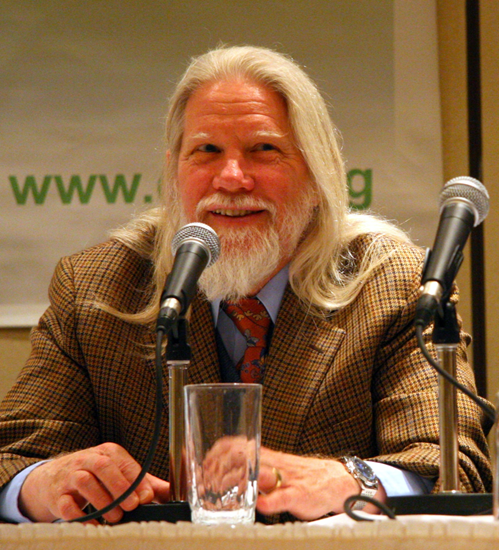
\includegraphics[scale = 0.4]{pictures/Bailey_Whitfield_Diffie.png}
% \end{figure}
% Bailey Whitfield 'Whit' Diffie\\ (sinh 05/06/1944 – 80 tuổi)
% \end{column}

% \begin{column}{0.4\textwidth}
% \begin{figure}[H]
% \centering
% 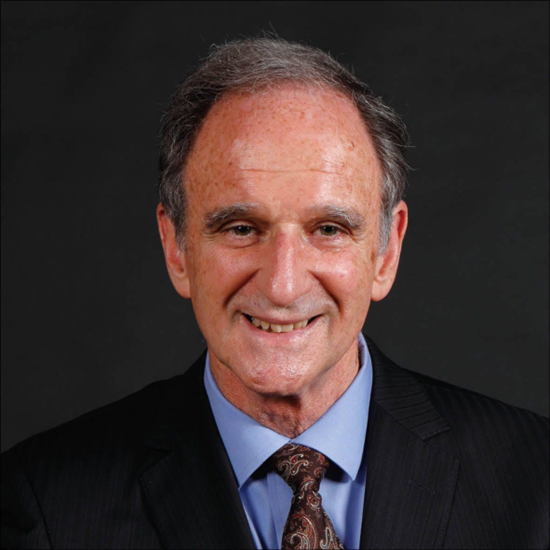
\includegraphics[scale = 0.4]{pictures/Martin_Edward_Hellman.png}
% \end{figure}
% Martin Edward Hellman\\(sinh 02/10/1945 - 79 tuổi)
% \end{column}

% \end{columns}
% \end{frame}
%%%%%%%%%%%%%%%%%%%%%%%%%%%%%%%%%%%%%%%%%%%%%%%%%%%%%%%
% \subsection{Khái niệm}
% \begin{frame}{Khái niệm}

% \begin{itemize}
% \item Hệ mật mã khóa công khai là một dạng mật mã hoá cho phép người sử dụng trao đổi các thông tin mật mà không cần phải trao đổi các khoá chung bí mật trước đó
% \item Việc mã hóa công khai được thực hiện bằng cách sử dụng một cặp khóa có quan hệ toán học với nhau là khóa công khai và khoá bí mật
% \begin{itemize}
% \item Khóa công khai: được công khai phổ biến - dùng để mã hóa
% \item Khóa bí mật: được giữ bí mật - dùng để giải mã
% \end{itemize}
% \end{itemize}

% $\Rightarrow$ Điều này đảm bảo hệ thống là không thể (hoặc rất khó) tìm ra khóa bí mật nếu chỉ biết khóa công khai

% \end{frame}
%%%%%%%%%%%%%%%%%%%%%%%%%%%%%%%%%%%%%%%%%%%%%%%%%%%%%%%
% \subsection{Mô hình tổng quát}
% \begin{frame}{Mô hình tổng quát}
% \begin{figure}[H]
% \centering
% 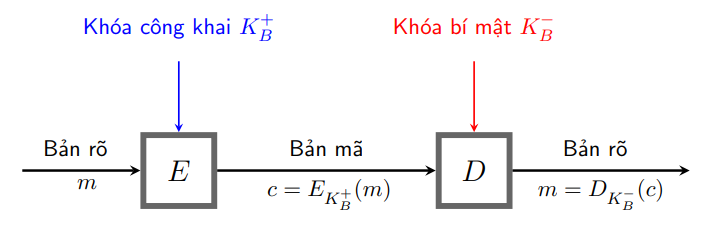
\includegraphics[scale = 0.6]{pictures/mo_hinh_tong_quat.png}
% \end{figure}
% \end{frame}
%%%%%%%%%%%%%%%%%%%%%%%%%%%%%%%%%%%%%%%%%%%%%%%%%%%%%%%

%! %%%%%%%%%%%%%%%%%%%%%%%%%%%%%%%%%%%%%%%%%%%%%%%%%%%%%%
%! %%%%%%%%%%%%%%%%%%%%%%%%%%%%%%%%%%%%%%%%%%%%%%%%%%%%%%
%! %%%%%%%%%%%%%%%%%%%%%%%%%%%%%%%%%%%%%%%%%%%%%%%%%%%%%%
%! %%%%%%%%%%%%%%%%%%%%%%%%%%%%%%%%%%%%%%%%%%%%%%%%%%%%%%
%! %%%%%%%%%%%%%%%%%%%%%%%%%%%%%%%%%%%%%%%%%%%%%%%%%%%%%%
% <!-- Giới thiệu về hệ mật mã Rabin -->
\section{Hệ mật mã RSA}
\subsection{xxxxxxxxxxxxxxxxxxxxxx}
\subsubsection{xxxxxxxxxxxxxxxxxxxxxx}
\begin{frame}{xxxxxxxxxxxxxxxxxxxxxx}

\end{frame}
%%%%%%%%%%%%%%%%%%%%%%%%%%%%%%%%%%%%%%%%%%%%%%%%%%%%%%%

%! %%%%%%%%%%%%%%%%%%%%%%%%%%%%%%%%%%%%%%%%%%%%%%%%%%%%%%
%! %%%%%%%%%%%%%%%%%%%%%%%%%%%%%%%%%%%%%%%%%%%%%%%%%%%%%%
%! %%%%%%%%%%%%%%%%%%%%%%%%%%%%%%%%%%%%%%%%%%%%%%%%%%%%%%
%! %%%%%%%%%%%%%%%%%%%%%%%%%%%%%%%%%%%%%%%%%%%%%%%%%%%%%%
%! %%%%%%%%%%%%%%%%%%%%%%%%%%%%%%%%%%%%%%%%%%%%%%%%%%%%%%
\section{Phương pháp lưới và thuật toán LLL giảm lưới}
\subsection{xxxxxxxxxxxxxxxxxxxxxx}
\subsubsection{xxxxxxxxxxxxxxxxxxxxxx}
\begin{frame}{xxxxxxxxxxxxxxxxxxxxxx}

\end{frame}
%%%%%%%%%%%%%%%%%%%%%%%%%%%%%%%%%%%%%%%%%%%%%%%%%%%%%%%
%! %%%%%%%%%%%%%%%%%%%%%%%%%%%%%%%%%%%%%%%%%%%%%%%%%%%%%%
%! %%%%%%%%%%%%%%%%%%%%%%%%%%%%%%%%%%%%%%%%%%%%%%%%%%%%%%
%! %%%%%%%%%%%%%%%%%%%%%%%%%%%%%%%%%%%%%%%%%%%%%%%%%%%%%%
%! %%%%%%%%%%%%%%%%%%%%%%%%%%%%%%%%%%%%%%%%%%%%%%%%%%%%%%
%! %%%%%%%%%%%%%%%%%%%%%%%%%%%%%%%%%%%%%%%%%%%%%%%%%%%%%%
% \section{Tổng kết}
% \subsection{Tổng kết}
% \subsubsection{Tổng kết}
% \begin{frame}{Tổng kết}
% Có cần phần Tổng kết????
% \end{frame}
%%%%%%%%%%%%%%%%%%%%%%%%%%%%%%%%%%%%%%%%%%%%%%%%%%%%%%%

%! %%%%%%%%%%%%%%%%%%%%%%%%%%%%%%%%%%%%%%%%%%%%%%%%%%%%%%
%! %%%%%%%%%%%%%%%%%%%%%%%%%%%%%%%%%%%%%%%%%%%%%%%%%%%%%%
%! %%%%%%%%%%%%%%%%%%%%%%%%%%%%%%%%%%%%%%%%%%%%%%%%%%%%%%
%! %%%%%%%%%%%%%%%%%%%%%%%%%%%%%%%%%%%%%%%%%%%%%%%%%%%%%%
%! %%%%%%%%%%%%%%%%%%%%%%%%%%%%%%%%%%%%%%%%%%%%%%%%%%%%%%
% \section*{}
% \begin{frame}{}
% \centering
% \Huge{Thanks for listening!}
% \end{frame}
%%%%%%%%%%%%%%%%%%%%%%%%%%%%%%%%%%%%%%%%%%%%%%%%%%%%%%%
\end{document}

% \begin{columns}

% \begin{column}{0.4\textwidth}
% \includegraphics[width=\textwidth]{pictures/Giới thiệu về HRM.png}
% \end{column}

% \begin{column}{0.6\textwidth}
% \begin{itemize}
% \item \dots
% \item \dots
% \item \dots
% \end{itemize}
% \end{column}

% \end{columns}